\documentclass[12pt,letterpaper,titlepage]{article}
%\usepackage[latin1]{inputenc}
\usepackage[spanish]{babel}


\usepackage[utf8]{inputenc}
\usepackage{ragged2e}
\usepackage{amsmath}
\usepackage{amsfonts}
\usepackage{amssymb}
\usepackage[none]{hyphenat}
\tolerance =3000
\pretolerance =2000

\usepackage[bookmarks]{hyperref}%,colorlinks,citecolor=black,linkcolor=black,urlcolor=black
\usepackage{appendix}
\usepackage{multirow}
\usepackage{graphicx}
%Modificar margenes
\usepackage{anysize}

\usepackage{fancyBOX}

%Para crear el encabezado y pie de pagina a nuestro gusto
\usepackage{fancyhdr}

% TABLA
\usepackage{dcolumn}
\usepackage{multirow}
\usepackage{slashbox}
\usepackage{rotating}
\usepackage{graphicx}

%COLOR
\usepackage{colortbl}

%Creamos el encabezado y pie de pagina
\pagestyle{fancy}
\fancyhf{}%Borra todas las configuraciones
\fancyhead[L]{\footnotesize \leftmark}%Alineado a la izquierda CAPITULO # %TITULO DE %CAPITULO
\fancyhead[R]{\footnotesize \thepage}%Alineado a la derecha numero de pagina
\fancyfoot[C]{\footnotesize \thepage}%Centrado numero de pagina
\renewcommand{\headrulewidth}{0.4pt}
\setlength{\headheight}{13pt}%Aumentamos el tama\~no del contenedor para el %encabezado

%Margenes izquierdo - derecho - superior - inferior
\marginsize{3cm}{2.7cm}{2.5cm}{2.5cm}
\author{Francisco Argüelles Granados}
\title{Estado del Arte}
\date{\today}
%%%%%%%%%%%%%%%%%%%%%%%%%%%%%%%% BEGIN DOCUMENT
\begin{document}

\textbf{}
%\maketitle
%\linebreak 
%\linebreak 
%\linebreak 
%
%\begin{center}
%\textit{Diseño de una plataforma web para el análisis de 
%cromosomas enfocado a la toma de decisiones.}
%\end{center}

%\newpage
\setlength{\unitlength}{1 cm} %Especificar unidad de trabajo
\thispagestyle{empty}
\begin{picture}(4,4)
\put(4.3,0){
\includegraphics[width=5cm,height=4cm]{itcv.jpg}}
\end{picture}
\\
\begin{center}
\textbf{{\Huge Instituto Tecnológico de Ciudad Victoria}\\[0.5cm]
{\large Maestría Profesionalizante en Sistemas Computacionales}}\\[1cm]
{\Large Protocolo de tesis}\\[1.3cm]
{\LARGE \textbf{Diseño de una plataforma web para el análisis de 
cromosomas enfocado a la toma de decisiones}}\\[1.5cm]
{\large Francisco Argüelles Granados}\\[1cm]
\textbf{Asesor de Tesis:}\\
Dr. Pedro Sánchez Orellana\\[0.7cm]
%{\large Beca:DGEST }\\[0.7cm]
Ciudad Victoria, Tamaulipas -  \today\

\end{center}


%%%%%%%%%%%
\newpage
\begin{center}
\tableofcontents
\end{center}
\newpage
\glossary{Resumen}
\section{Resumen}\label{resumen}
%\subsection{Resumen}
Nuestro mundo actual está prominentemente dominado por la tecnología, vivimos en una sociedad donde los avances tecnológicos, son parte de nuestra vida diaria y muchas veces dependemos de ellos para poder llevar a cabo nuestras actividades cotidianas.\\

%\end{quotation}
%\begin{quotation}
Muchos avances tecnológicos han venido a ayudar a otras áreas como la economía y el arte, por mencionar a algunas, y sin lugar a dudas el sector salud ha sido también beneficiado con diversos equipos tecnológicos que sirven de apoyo a esta área, tanto a nivel local, nacional y mundial.\\

Aun y cuando esta tecnología nos ayuda a proporcionar servicios para atención y prevención de enfermedades hereditarias, los equipos diseñados con este fin son demasiado caros y pocos son los hospitales y centros de salud que los poseen y cuentan con personal calificado para su operación, lo que ocasiona que el servicio de cariotipo -tema de esta propuesta de tesis- tenga un costo elevado y que para algunas personas no es tan fácil poderlo realizar, como por ejemplo a la población que habita en zonas rurales no le es tan fácil desplazarse a las grandes ciudades donde por lo regular se realiza este tipo de estudio.\\

Es aquí donde se pretende aprovechar los avances tecnológicos, principalmente el uso de Internet donde se puede tener acceso en la mayor parte del país incluyendo las zonas rurales; esto con el fin poder establecer un Servicio Web que permita realizar el cariotipo y generar un reporte que apoye al diagnóstico del médico en cuestión.\\

%%%%%%%%%%%%%%%%%%%%%%% INTRODUCCION
%\newpage
%\glossary{Introduccion}
\section{Introducción}\label{intro}
%\subsection{Introducción}
%\begin{quotation}
La presente propuesta de tesis está enfocada a proporcionar una herramienta computacional, enfocada a la toma de decisiones en el sector salud. De manera más específica, en el rubro de diagnóstico de laboratorio e imagenología. El producto que se espera obtener, es un servicio web auxiliar en el diagnóstico temprano de enfermedades genéticas. El cariotipo es un esquema o imagen de los cromosomas de una célula metafásica, ordenados de acuerdo a su morfología y tamaño. Mediante el proceso de cariotipado se pueden analizar diversas anomalías cromosómicas. En el Hospital Infantil de Tamaulipas (HIT) se ha utilizado dicho proceso para detectar algunas anomalías cromosómicas como el Síndrome de Turner \footnote{turnersyndrome.org}, de Klinefelter \footnote{klinefeltersyndrome.org}, de Betwith-Wiedeman \footnote{beckwith-wiedemannsyndrome.org}, de Down \footnote{ds-int.org} y de Prader Willi \footnote{pwsausa.org}. Todos estos síndromes son altamente discapacitantes y reducen la calidad y el tiempo de vida de las personas afectadas. \\


Estos análisis cromosómicos se realizan a partir de una muestra de sangre o de tejido. Para poder observar los cromosomas con un microscopio, la muestra debe ser teñida y fotografiada. A partir de esa fotografía, un experto puede separar y organizar los cromosomas de acuerdo a su forma y tamaño. Esta tarea requiere de varios días para ser completada. Debido a la gran cantidad de tiempo que implica la realización de este estudio, algunas compañías han comercializado herramientas computacionales que permiten reducir el tiempo de realización de un cariotipo. Estas herramientas requieren generalmente que el usuario inicialice el proceso de segmentación y clasificación y están desarrolladas bajo código cerrado, lo que no permite su adaptación a las necesidades del usuario final. \\


Actualmente, el departamento de citogenética del HIT realiza estudios genéticos basados en cariotipos efectuados en forma manual, lo que implica tiempos de diagnóstico muy elevados, de cuando menos 12 horas, y por lo tanto un número reducido de estudios por mes. La división de estudios de posgrado e investigación (DEPI), en la maestría de sistemas computacionales, en el Instituto Tecnológico de Ciudad Victoria (ITCV), propone desarrollar un servicio web que permita a distintas instituciones realizar el cariotipo automáticamente a partir de imágenes obtenidas en microscopía convencional y auxilie en el diagnóstico temprano de enfermedades genéticas. Este sistema tendrá la particularidad de funcionar en Internet, permitiendo a múltiples instituciones de salud realizar dichos análisis en cuestión de minutos. Lo anterior se traduce en un incremento en la cantidad de pacientes con posibles anomalías genéticas. \\


%%%%%%%%%%%%%%%%%%%%%%% ANTECEDENTES
%\newpage
\section{Antecedentes}\label{antecedentes}
%\begin{quotation}
Los defectos de nacimiento y las enfermedades genéticas son causa importante de mortalidad infantil y representan un problema de salud pública. Bertina et al. en 2009 \cite{102} muestra que las enfermedades genéticas y los defectos de nacimiento constituyen entre el 40\% y el 50\% de las causas de hospitalización pediátrica en hospitales y centros de alta especialidad, cifra que se incrementa considerando los múltiples internamientos a los que pueden estar sujetos estos pacientes. En México, según el informe del Consejo Nacional de Población (CONAPO) \cite{101}, las enfermedades congénitas han aumentado a partir de 1997 y desde entonces ocupan el segundo lugar como causa de mortalidad infantil. El Instituto Nacional de Estadística y Geografía (INEGI) señaló en el año 2006 que las malformaciones congénitas, las deformidades y las anomalías cromosómicas son la segunda causa de muerte en niños de uno a cuatro años, la tercera en niños de cinco a 14 años y como causa de morbilidad general ocupa el número 20 \cite{102}. El Instituto Nacional de Pediatría \footnote{Anuario Estadístico 2007}informó que las enfermedades congénitas presentan una tasa de 11.2\% de pacientes atendidos como causa de consulta de primera vez, la más alta para dicho periodo. \\
%\end{quotation}

%\begin{quotation}
En el estado de Tamaulipas en 2007 \footnote{Secretaría de Salud 2007}, la tasa de natalidad es de 18.53 nacimientos por cada 1000 habitantes, de los cuales, 3\% presentará alguna malformación congénita. En Tamaulipas, el 65.05\% de los tamaulipecos son atendidos por instituciones de seguridad social y el 34.95\% por los servicios de salud para población abierta\footnote{INEGI. Encuesta Nacional de Empleo y Seguridad Social 2009. Aguascalientes, Ags., México. 2010}, al cual pertenece el Hospital Infantil de Tamaulipas (HIT). En el HIT, en el área de citogenética, debido a la integración de médicos especialistas de tiempo completo en las áreas de Genética, Hematología y Oncología, entre los años 2007 y 2009 el número de consultas y de estudios de cariotipo al mes asciende a 39 en promedio (cifra que se mantiene durante los últimos años). En estas áreas médicas, gran parte de los diagnósticos de enfermedades genéticas se realizan por medio de estudios de cariotipo basados en el análisis de fotografías obtenidas por microscopía. \\
%\end{quotation}

%\begin{quotation}
Un cariotipo es un esquema o imagen de los cromosomas de una célula metafásica, ordenados de acuerdo a su morfología y tamaño (ver Apéndice A). Algunos ejemplos de anomalías cromosómicas que se han detectado en el HIT son el Síndrome de Turner, de Klinefelter, de Betwith-Wiedeman, de Down y de Prader Willi. Todos estos síndromes son altamente discapacitantes y reducen la calidad y el tiempo de vida de las personas afectadas. Estos análisis cromosómicos se realizan a partir de una muestra de sangre o de tejido que es teñida y fotografiada mediante una cámara adaptada a un microscopio. A partir de la fotografía tomada, un experto puede separar y organizar los cromosomas de acuerdo a su forma y tamaño, los cual requiere de varios días para ser completada. Debido a la gran cantidad de tiempo requerido para la realización de este estudio, se han comercializado herramientas computacionales que permiten reducir el tiempo de realización de un cariotipo. El costo de estas herramientas es muy elevado (alrededor de 250,000 pesos, solamente el software de procesamiento, según una cotización facilitada por personal del HIT) y están desarrolladas bajo código cerrado, lo que no permite su adaptación a las necesidades del usuario final. Actualmente, el departamento de citogenética del HIT realiza estudios genéticos basados en cariotipos, que son obtenidos en forma manual, lo que acarrea tiempos de diagnóstico prolongados y consecuentemente, un número reducido de estudios por mes. \\
%\end{quotation}
%\begin{quotation}
Los médicos de las áreas de Genética, Oncología y Hematología del HIT han expresado que la falta de un equipo que facilite el procesamiento de imágenes automatizadas y de técnicas que contribuyan a la emisión de diagnósticos más precisos, hace que en los pacientes con enfermedades genéticas y hemato-oncológicas como las leucemias, tengan que ser referidos a centros hospitalarios foráneos que cuentan con equipo especializado para el análisis genéticos, lo que implica un alto impacto económico en traslado y pago de servicios para los pacientes. Así mismo, expresaron que ésta referencia de pacientes a laboratorios externos especializados podría disminuir si el Laboratorio de Citogenética del HIT contara con un sistema que generara cariotipos en forma automatizada, además de que se podría atender a un mayor número de pacientes por mes. \\


Para atender esta necesidad, la división de estudios de posgrado e investigación del ITCV en colaboración la división de investigación del HIT e investigadores de la Universidad Politécnica de Victoria (UPV), propone desarrollar un servicio web para el procesamiento computacional de imágenes de cromosomas que genere cariotipos sin intervención humana a partir de imágenes obtenidas en microscopia convencional. La finalidad de dicho servicio web es brindar una herramienta de fácil uso, durante el proceso de diagnóstico temprano de enfermedades genéticas. Debido a que este sistema será desarrollado por investigadores nacionales con tecnología flexible y de funcionamiento en internet, el análisis podría ser aplicado en cualquier centro hospitalario de la Secretaría de Salud que así lo requiera (y que cuente con las herramientas de microscopia necesarias). Una vez terminada la etapa de investigación y desarrollo básica, se tendrá un costo menor comparado con el de los sistemas comerciales. Además, ya que el sistema generará un cariotipo en un tiempo notoriamente menor (alrededor de 10 minutos) comparado con el tiempo tomado por el método manual, las áreas de Genética, Oncología y Hematología del centro hospitalario donde sea instalado podrán aumentar su capacidad de atención a pacientes. \\
%\end{quotation}

%%%%%%%%%%%%%%%%%%%%%%% MARCO TEORICO

\section{Marco teórico}\label{marco}
%\begin{quotation}
Con respecto a las técnicas de procesamiento y análisis de imágenes que serán exploradas para el desarrollo del proyecto, se consultarán referencias bibliográficas comunes que contienen información de operadores y algoritmos para procesar y analizar imágenes. Por ejemplo, en  González \cite{1077}, se tratan fundamentos y técnicas relacionadas con el análisis y procesamiento de imágenes desde una perspectiva general. En relación al análisis y procesamiento de imágenes aplicadas a imágenes de microscopia, en Castleman \cite{1022} se reportan un conjunto de técnicas generales que han dado muy buenos resultados para esa clase particular de imágenes. Con respecto al análisis de imágenes de cromosomas y obtención de cariotipo, se han reportado soluciones desde enfoques muy variados. Uno de los enfoques más importantes es el enfoque basado en clasificación \cite{113}, en donde se intenta segmentar los cromosomas utilizando herramientas de aprendizaje automático. Un enfoque comúnmente utilizado está basado en redes neuronales artificiales \cite{104} \cite{111}, en donde se aplica un conjunto de operadores de procesamiento de imagen y la clasificación de los cromosomas se  realiza mediante una red neuronal. El mejoramiento de la imagen es una etapa de procesamiento digital en donde se aplican un conjunto de operadores que permiten eliminar el ruido de la imagen derivado del proceso de adquisición, así como realizar ciertas correcciones a la iluminación \cite{114}. La segmentación es también una fase importante del procesamiento que debe ser aplicado a las imágenes, en donde la finalidad es la separación de regiones de interés, cromosomas en nuestro caso, del resto de la imagen \cite{106} \cite{109} \cite{103} \cite{117} \cite{112}. Se han propuesto también técnicas de segmentación basadas en la transformada Wavelet \cite{116} \cite{115}. \\
%\end{quotation}

%\begin{quotation}
En el caso de la propuesta del Dr. Yahir Hernández y el Dr. Pedro Sánchez se hace uso de una arquitectura como la mostrada en la Figura 1, cuyas etapas se describen a continuación:\\\\

\begin{figure}
  \centering
    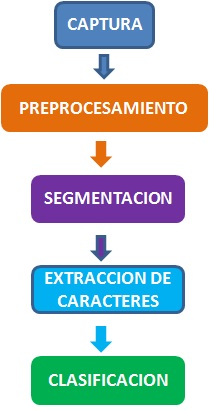
\includegraphics[width=0.2\textwidth]{EsquemaBasicoRecPatronesPrev}
  \caption{Arquitectura propuesta.}
  \label{fig1:SW}
\end{figure}
%\end{quotation}

\begin{itemize}\itemsep=0pt
\item  \textbf{Captura.-} Consiste en obtener la imagen de las cromosomas(Figura 2).
\begin{figure}
  \centering
    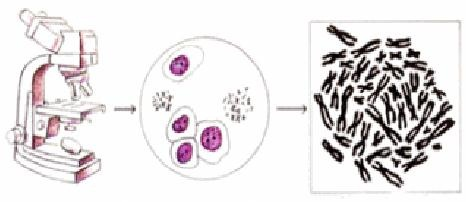
\includegraphics[width=0.4\textwidth]{1_Captura}
  \caption{Etapa de captura de los cromosomas.}
  \label{fig2:EBRP}
\end{figure}

\item  \textbf{Preprocesamiento.-} Consiste en analizar la imagen obtenida en la etapa anterior, eliminando la información irrelevante (o ruido) para el estudio.
\item  \textbf{Segmentación.-} Permite la diferenciar entre los cromosomas y el fondo dentro de la metafase celular. La segmentación consta de las etapas de binarización, la limpieza de objetos e impurezas, la separación de cromosomas unidos o traslapados y la corrección de algunos cromosomas recortados o incompletos producto de la binarización inicial.
\item  \textbf{Extracción de características.-} En esta fase se escogen las características a extraer de las imágenes de los cromosomas segmentados en la fase anterior, para crear la matriz de características que se usará para crear y entrenar el modelo de clasificación.\\
La primera característica que buscan los expertos a la hora de realizar el cariotipado es el tamaño. Dependiendo del tamaño son capaces de clasificar los cromosomas en pequeños grupos. \cite{131}. Después buscan características como el índice del centrómero (ratio entre el brazo corto del cromosoma y la longitud total) o la posición de las bandas características. Con este método el experto puede hacer el cariotipado de manera fiable.
\item  \textbf{Clasificación.-} En el cariotipo humano se ha establecido en grupos de cromosomas.\\

%\end{quotation}


%\begin{quotation}
Finalmente, la implementación de estas etapas se realizará mediante algunas herramientas de desarrollo de código libre que incluyen un marco de trabajo que representa una alternativa importante con respecto al software comercial. Con estas herramientas es posible desarrollar proyectos de investigación interesantes sin que esto represente un desembolso significativo para las instituciones participantes. Una alternativa de herramientas de código libre es el OpenCV (Open Computer Vision), la cual es una biblioteca multiplataforma libre que contiene una gran cantidad de operadores de procesamiento digital de imágenes. Con respecto a esta herramienta,  Kaehler \cite{110} es una referencia bibliográfica muy importante dado que documenta ampliamente el uso de los componentes de la biblioteca. Otra de las herramientas de código libre que podría ser utilizada para la parte de clasificación requerida en el proyecto es WEKA (Waikato Environment for Knowledge Analysis), la cual es un software para aprendizaje automático y minería de datos. Una de las referencias más citadas con respecto a esta herramienta es Frank \cite{105}, la cual ha sido ampliamente consultada en diferentes artículos como una referencia importante con respecto a los algoritmos de clasificación disponibles en esta herramienta.\\
%\end{quotation}

%\begin{quotation}
Dado que el uso de este tipo herramientas computacionales es de gran utilidad para la sociedad es importante que diferentes servicios de salud tengan acceso a él.\\

Para realizar el proceso de análisis se propone el uso de un Servicio Web el cual se utilizará para que se pueda subir la imagen a analizar, poder procesarla y regresar los resultados en reporte en archivo PDF.\\
%\end{quotation}

%\begin{quotation}
Las ventajas que se tienen de realizar el proceso de esta manera son las siguientes:
%\end{quotation}

\begin{itemize}\itemsep=0pt
\item  Se puede atender a cualquier hora sin necesidad de tener a una persona dedicada a la realización del proceso de segmentación de la imagen enviada.\\
\item No es necesario que el paciente o la persona que requiera hacer el análisis se tenga que trasladar de su localidad, ya que el servicio de intenet se ha extendido 
ampliamente en el territorio nacional llegando a poblaciones rurales donde no existen centros de salud especializados.\\
\item El punto anterior nos lleva a un ahorro en gastos de transportación y alimentación que tendrían que desembolsar las personas si quisieran trasladarse a un centro de salud que lleve a cabo este proceso.\\
\item Los servicios de salud pueden hacer uso del Servicio Web para beneficio de sus derechohabientes.\\
\end{itemize}

%\begin{quotation}
Antes de continuar, vamos a definir el concepto básico de un "Servicio Web". Un servicio web es una interfaz de red que puede acceder a la funcionalidad de una aplicación, usando tecnologías de Internet (ver Apéndice B). \\ % \cite{119}\\
%\end{quotation}



%\begin{quotation}
Debido a que en este proyecto el objetivo es que cualquier persona pueda subir una imagen de un cariotipo y mediante un procesamiento e interacción con un servicio Web se pueda obtener un reporte del cariotipo analizado se va a usar un Servicio Web para Análisis (WSA).\\
%\end{quotation}

%\begin{quotation}
Para lograr lo comentado, se utilizará un esquema cliente - servidor como se muestra en la Figura 3, a realizar compresión de imágenes. Las imágenes se han convertido en un área muy importante de la informática. Hoy en día surgen más entornos gráficos orientados a múltiples aplicaciones. El uso de las imágenes se ha incrementado con el desarrollo de la informática, de igual forma su resolución (y por tanto tamaño), de ahí la necesidad de compactarlas para reducir la cantidad de datos a enviar por la web. La compresión (Paso 1, Figura 3)se basa en la eliminación de datos redundantes; dicho de otra forma, equivale a transformar una distribución bidimensional de pixeles en un conjunto de datos estadísticos sin correlacionar. Esta transformación (compresión) es aplicada a las imágenes antes de que sean almacenadas o antes de ser enviadas, por ejemplo vía red o internet. \\
%\end{quotation}

%\begin{quotation}
Con la compresión de imágenes se trata de minimizar el número de bits para representar una imagen. Las aplicaciones de la compresión de imágenes son principalmente la transmisión y almacenamiento de información. En trasmisión, sus principales aplicaciones son la televisión, el radar, redes de computadoras entre otras. En almacenamiento, la compresión de imágenes se utiliza sobre documentos, imágenes de satélite, imágenes médicas. Debido a lo comentado es que se requiere un procedimiento para realizar la compresión para su envío mediante un Servicio Web  (Paso 2, Figura 3) y sin pérdida de información relevante, y así poder llevar a cabo el cariotipo. El flujo de funcionamiento de la aplicación se muestra en la figura 3. \\

\begin{figure}
  \centering
    \includegraphics[width=0.9\textwidth]{FlujoFuncionamiento2}
  \caption{Flujo de funcionamiento de la aplicación}
  \label{fig3:FFA}
\end{figure}
%\end{quotation}

%\begin{quotation}
El Servicio Web tendrá una interacción con el proceso investigadores de la Universidad Politécnica de Victoria (UPV) en conjunto con investigadores del Hospital Infantil de Tamaulipas (HIT).\\
%\end{quotation}

%\begin{quotation}
Una vez que la imágen llega al servidor donde se encuentra instalada la aplicacion para la realización del cariotipo, se procede a descomprimir la imagen que fue comprimida durante el envío (Paso 3, Figura 3). El prepocesamiento (Paso 4, Figura 3) consiste en el alizado de la iluminación, debido a que las imágenes tienen desmedrada la iluminación y contienen ruido.\\
%\end{quotation}

%\begin{quotation}
Con la segmentación (Paso 4, Figura 3) se hace la evaluación geométrica de los cromosomas y sus intersecciones para lograr la separación de los mismos. La extracción de características (Paso 5, Figura 3) lleva a cabo la evaluación de los niveles de intensidad de los cromosomas para eliminar el ruido. Esto se genera en señales de entrenamiento.\\
%\end{quotation}

%\begin{quotation}
La forma de realizar la clasificación (Paso 6, Figura 3), se explicará más adelante dentro del Marco Teórico.\\
%\end{quotation}


%\begin{quotation}
Una vez obtenido el cariotipo (ver Figura 4), se procederá a generar un reporte de apoyo a la toma de decisiones del médico solicitante del estudio.\\
%\end{quotation}

\begin{figure}
  \centering
    \includegraphics[width=0.6\textwidth]{CariotipoHumano1}
  \caption{Cariotipo Humano}
  \label{fig5:CariotipoHumano}
\end{figure}


%\begin{quotation}
Para elaborar el cariotipado es importante la clasificación de los cromosomas segmentados. El proceso a realizar en esta propuesta de tesis utiliza las redes neuronales, las cuales se describen a continuación:\\
%\end{quotation}

%\begin{quotation}
Debido a que el cariotipo es una forma de análisis cromosómico que se basa en el ordenamiento estándar de los cromosomas contenidos en una célula, de acuerdo con su tamaño, localización del centrómetro \footnote{Región del cromosoma que separa los dos brazos y en la que se unen las dos cromátides. Es la región de unión a las fibras del huso acromático durante la división celular.} y patrón de bandeo \footnote{Por patrón de Bandeo se entiende el conjunto de bandas transversales de tamaño en intensidad de tinción diferentes que aparecen sobre cromosomas determinados según el modelo de distribución que depende del tinte utilizado}, éste será realizado por los investigadores de la UPV.\\

Posteriormente se realizará el proceso de clasificación. Existen diferentes tipos de técnicas para la clasificación de cromosomas por ejemplo Benoit Legrand et al. \cite{132}, proponen la técnica basada en tiempo de deformación dinámico para determinar la longitud y el perfil de densidad que son características comunes que se utilizan en la clasificación de los cromosomas.\\

Gunter Ritter \cite{133} se basa en una combinación de dos fases, una fase puramente basado en reglas y una fase impulsada por análisis discriminante restringida, pero con la desventaja que no puede realizar la clasificación de los cromosomas con información parcial, que sucede cuando los cromosomas se ocluyen entre si, por otro lado se propone el uso de redes neuronales artificiales:\\
%\end{quotation}

%\begin{quotation}
Las redes neuronales tambien denominadas redes neuronales artificiales (RNA)son sistemas ideados como abstracciones de las estructuras neurobiológicas (cerebros) encontradas en la naturaleza y tienen la característica de ser sistemas desordenados capaces de guardar información.
 \footnote{info.fisica.uson.mx/arnulfo.castellanos/archivos/html/quesonredneu.htm}\\
%\end{quotation}

%\begin{quotation}
No existe un definición general de una red neuronal artificial, existiendo diverentes según el texto ó artículo consultado; de las que podemos mencionar:
%\end{quotation}

\begin{itemize}\itemsep=0pt
\item Una red neuronal es un modelo computacional, paralelo, compuesto de unidades procesadoras adaptativas con una alta interconexión entre ellas.  \cite{126}\\
\item Modelos matemáticos desarrollados para emular el cerebro humano. \cite{127}\\
\item Sistema de procesamiento de información que tiene características de funcionamiento comunes con las redes neuronales biológicas. \cite{128}\\
\end{itemize}


%\begin{quotation}
Las RNA al margen de parecerse al cerebro presentan una serie de características
propias del cerebro. Por ejemplo las RNA aprenden de la experiencia, generalizan de
ejemplos previos a ejemplos nuevos y abstraen las características principales de una
serie de datos. \cite{124}
%\end{quotation}

\begin{itemize}\itemsep=0pt
\item  \textbf{Aprender.-} Adquirir el conocimiento de una cosa por medio del estudio, ejercicio
o experiencia. Las RNA pueden cambiar su comportamiento en función del entorno. Se
les muestra un conjunto de entradas y ellas mismas se ajustan para producir unas salidas
consistentes.
\item  \textbf{Generalizar.-} Extender o ampliar una cosa. Las RNA generalizan
automáticamente debido a su propia estructura y naturaleza. Estas redes pueden ofrecer,
dentro de un margen, respuestas correctas a entradas que presentan pequeñas
variaciones debido a los efectos de ruido o distorsión.
\item  \textbf{Abstraer.-} Aislar mentalmente o considerar por separado las cualidades de un
objeto. Algunas RNA son capaces de abstraer la esencia de un conjunto de entradas que
aparentemente no presentan aspectos comunes o relativos.
\end{itemize}

%%\begin{quotation}
%El modelo de funcionamiento de una neurona real se presenta en la Figura 5. \\
%%\end{quotation}
%
%%\begin{quotation}
%Matemáticamente su representación  se  puede ver en la Figura 6. \\
%%\end{quotation}
%
%
%\begin{figure}
%  \centering
%    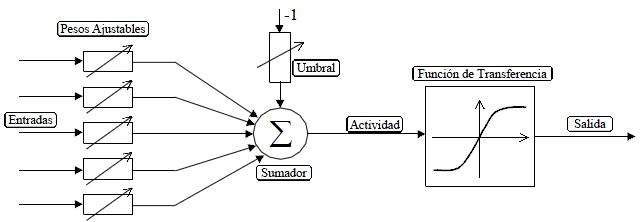
\includegraphics[width=0.9\textwidth]{ModeloNeurona}
%  \caption{Modelo de funcionamiento de una neurona real}
%  \label{fig5:MN}
%\end{figure}
%
%
%\begin{figure}
%  \centering
%    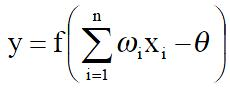
\includegraphics[width=0.3\textwidth]{ModeloNeuronaFormula}
%  \caption{Modelo de Neurona Entrada/Salida}
%  \label{fig6:MN}
%\end{figure}

%\begin{quotation}
La estructura de la red neuronal le permite la resolución de problemas que necesitarían gran cantidad de tiempo en computadoras comunes. Aparte de este hecho aparecen propiedades que las hacen atractivas para ser usadas en una gran cantidad de problemas prácticos \cite{125}
%\end{quotation}

\begin{itemize}\itemsep=0pt
\item  \textbf{Son sistemas distribuidos no lineales.-} Una neurona es un elemento no lineal por lo que una interconexión	 de ellas (red neuronal) también será un dispositivo no lineal. Esta propiedad permitirá la simulación de sistemas no  lineales y caóticos, simulación que, con los sistemas clásicos lineales, no se puede realizar.
\item  \textbf{Son sistemas tolerantes a fallas.-} Una red neuronal, al ser un sistema distribuido, permite el fallo de algunos elementos individuales (neuronas) si alterar significativamente la respuesta total del sistema.
\item  \textbf{Adaptabilidad.-} Una red neuronal tiene la capacidad de modificar los parámetros de los que depende su funcionamiento de acuerdo con los cambios que se produzcan en su entorno de trabajo (cambios en las entradas, presencia de ruido, etc).
\item  \textbf{Establecen relaciones no lineales entre datos.-} Las redes neuronales son capaces de relacionar dos conjuntos de datos. Comparando con los métodos estadísticos clásicos que realizan la misma misión tienen como principal ventaja que los datos no tienen por que cumplir las condiciones de linealidad, gausianidad y estacionariedad. \cite{129}
\item  \textbf{Posibilidad de implementación en integración en escala muy grande.-} Esta posibilidad permite que estos sistemas puedan ser aplicados en sistemas de tempo real, simulando sistemas biológicos mediante elementos de silicio. \cite{130}
\end{itemize}

%\begin{quotation}
Hasta aqui se ha presentado la parte principal de esta propuesta de tesis, se ha visto la forma en que se va a interactuar con los investigadores de la Universidad Politécnica de Victoria (UPV) y los investigadores del Hospital Infantil de Tamaulipas (HIT).\\

Como se mencionó anteriormente el servicio web (Web Service) que se va a implementar cumple la función de realizar la compresión/descompresión de la imagen de los cromosomas para poder transferirlo al proceso realizado por los investigadores de la UPV y posteriormente generar el estidio del cariotipo.
%\end{quotation}

%%%%%%%%%%%%%%%%%%%%%%% PLANTEAMIENTO DEL PROBLEMA

\section{Planteamiento del problema}\label{planteamientoproblema}


%\begin{quotation}
Como se vió en el marco teórico (sección 4. Marco teórico), el análisis de cromosomas (cariotipo) es un proceso lento el cual se lleva a cabo en aproximadamente 12 horas de trabajo, debido a la falta de herramientas automáticas que simplifiquen esta tarea; en consecuencia la cantidad de cariotipos que pueden realizarse es baja. Si a esto se le añade el costo de microscopios especializados este análisis se vuelve prohibitivo para comunidades rurales o marginadas cuyos centros de salud poseen en el mejor de los casos microscopios con características básicas. Por ello, los pacientes se ven forzados a desplazarse a las ciudades cercanas (lo cual implica un alto costo de traslado, alimentación, etc.) para realizar dicho análisis.\\
%\end{quotation}

%\begin{quotation}
Para resolver esta problemática, se plantea desarrollar un servicio web que permita la transmisión de $n$ imágenes de cromosomas de una persona a través de Internet y regrese los resultados, todo mediante una página web. Dicha tarea no es sencilla, pues cada imagen es superior a los $500kb$ y considerando la velocidad del servicio de las comunicaciones en zonas rurales no es buena y la eficiencia en dicha transmisión se convierte en una prioridad.\\
%\end{quotation}

%\begin{quotation}
Debido a los detalles mencionados anteriormente, se desarrollará un servicio Web para atender esta problemática donde se pretende cubrir los siguientes puntos:\\
%\end{quotation}


\begin{itemize}  %\itemsep=0pt
\item  Integrar un Servicio Web disponible para cualquier Centro de Salud principalmente los ubicados en zonas rurales.
\item  Que las Instituciones y Centros de salud públicos puedan realizar el estudio de cariotipo sin tener que invertir cantidades elevadas de dinero en instrumentación especializada. Este estudio se podrá realizar solamente contando con un microscopio con características básicas en un precio entre 50,000 y 70,000.00 M.N.
\item  Establecer un proceso de empaquetamiento para la imagen del cariotipo, que permita poder transferir la imagen lo más rápido posible considerando zonas rurales donde la velocidad y los métodos para conectarse a Internet dependan de dispositivos de baja velocidad de transmisión, por ejemplo un modem cuya máxima capacidad de transmisión es de 56 kbps.
\end{itemize}


%%%%%% 


%%%%%%%%%%%%%%%%%%%%%%% HIPOTESIS

\section{Hipótesis}\label{hipotesis}

%\begin{quotation}
%Hipótesis
%\end{quotation}

%\begin{quotation}
Debido que este tipo de análisis se realiza en ciudades grandes que cuentan con Instituciones y Centros de Salud de alta especialidad, pero que a su vez implica un mayor costo en los servicios que ofrecen al público en general, genera un costo considerable para las personas que viven en el campo, ya que deben de realizar gastos de traslado y alimentación a las ciudades donde se encuentran estos centros de salud u hospitales que cuentan con este servicio de análisis cromo somático.\\
%\end{quotation}

%\begin{quotation}
El uso de herramientas web para el análisis de cromosomas permite reducir los costos del análisis tradicional al permitir realizar el análisis utilizando microscopios de bajo costo, por lo que es más accesible para la población acercarse a un centro comunitario de salud a tener que realizar traslados a una ciudad lejos de su comunidad.\\
%\end{quotation}


%%%%%%%%%%%%%%%%%%%%%%% OBJETIVOS

\section{Objetivos}\label{objetivos}

La presenta propuesta de tesis contempla:\\

\textbf{Objetivo general.}\\

\begin{itemize}\itemsep=0pt
\item Desarrollar e implementar un sistema computacional flexible que utilice un Servicio Web, amigable para el usuario, auxiliar en el diagnóstico de enfermedades genéticas, que sea capaz de generar cariotipos automáticamente aplicando algoritmos de procesamiento digital en imágenes obtenidas en procedimientos cito genéticos estándar y cuyos resultados de clasificación sean similares a los obtenidos por un experto.\\
\end{itemize}

\textbf{Objetivos específicos.}\\

\begin{itemize}\itemsep=0pt
\item Implementar un Servicio Web para el procesamiento de las imágenes que se utilizarán para el estudio del cariotipo.
\item Implementar un mecanismo de compresión de imágenes que permitan su fácil transferencia al proceso de análisis de la misma.
\item Implantar el sistema propuesto en un centro hospitalario.
\end{itemize}


%%%%%%%%%%%%%JUSTIFICACION
\section{Justificación}\label{Justi}

Debido a que las Instituciones y Centros de Salud públicos cuentan con recursos limitados para su operación, por lo tanto la adquisición de equipo para realizar el cariotipo (microscopio y el software para su operación) no resulta viable. Es por esta razón que muchos pacientes se ven obligados a recibir este servicio en centros de salud privados o en centros de salud en otras ciudades, que en ambos casos implica un costo que la mayoría de ellos no pueden solventar.\\

Es por esta razón que nuestra propuesta de tesis considera el desarrollo de una plataforma web que permita a distintos centros de salud pública realizar cariotipos (empleando microscopios con tecnología básica).\\



%%%%%%%%%%%%% LIMITACIONES...
\section{Alcances y limitaciones}\label{limitaciones}

La presente propuesta de tesis se limitará a:

\begin{itemize}\itemsep=0pt
\item Proveer una herramienta web para cariotipo exclusivamente.
\item Proporcionar una herramienta que permita acelerar la transferencia de las imágenes mediante una técnica de compresión.
\item Proporcionar un Servicio Web que procese, reciba y descomprima las imágenes para finalmente elaborar un informe. Dicho informe servirá como una herramienta de apoyo al diagnóstico médico.
\item Para la generación del cariotipo se definirá un umbral mínimo de calidad de las imágenes de entrada (separación entre cromosomas y resolución).
\end{itemize}


%%%%%%%%%%%%%%%%%%%%%%% METODOLOGIA
\section{Metodología de investigación}\label{metodo}

La metodología de investigación que se seguirá durante el desarrollo de la presente propuesta de tesis se divide en 2 etapas:

\begin{itemize}
\item Durante la primera se investigará acerca de los tipos de servicios web, las estrategias y el software requerido existentes para su implementación. En este punto se revisarán las arquitecturas existentes para SOAP y REST. Así mismo, durante el desarrollo de esta etapa se montará un servidor local para realizar la implementación y las pruebas. Para ello se revisará la tecnología Linux ya que es de uso libre. Finalmente se iniciará con la investigación de las técnicas de compresión de imágenes existentes que permitirá agilizar la transferencia de imágenes entre el cliente y el servicio web; y se seleccionará la red neuronal a utilizar.\\

\item En la segunda etapa del proyecto se investigará sobre los métodos de compresión de imágenes, primeramente analizando los diversos métodos  existentes en la actualidad para determinar el método más adecuado que nos permita realizar una compresión de calidad y que ocupe pocos bytes de espacio. Una vez terminada la compresión de imágenes se implementará el módulo de clasificación (red neuronal) en el servidor, posteriormente se procederá a integrarlo con el servicio web para empezar a realizar las pruebas de la aplicación de cariotipo. En éste punto podemos empezar a elaborar el manual para que el usuario pueda realizar el cariotipo, con éste proyecto para finalmente implantar el sistema en el HIT.\\

\end{itemize}


%%%%%%%%%%%%%%%%%%%%%%% CRONOGRAMA

\section{Cronograma de actividades}\label{cronograma}
%\begin{quotation}
%Cronograma de Actividades
%\end{quotation}



\begin{center}
%\begin{sideways}
\scalebox{0.75}{
\begin{tabular}{|l|c|c|c|c|c|c|}
\hline
\textbf{\centering Actividad} & \textbf{Bim-I} & \textbf{Bim-II} & \textbf{Bim-III} & \textbf{Bim-IV} & \textbf{Bim-V} & \textbf{Bim-VI} \\
\hline
Investigar Estado del Arte (Cariotipado) & \cellcolor{black} & \cellcolor{black} &   &   &   &  \\ 
\hline
Investigación sobre Servicios Web &  & \cellcolor{black} &  \cellcolor{black}  &   &   &  \\
\hline
Inv. Métodos de Compresión de Imágenes & \cellcolor{black} &  \cellcolor{black} &  &  &  &  \\
\hline
Implementación del WebService &   &  & \cellcolor{black} &    &    &  \\
\hline
Implementación del Métodos de Compresión &   &   & \cellcolor{black} &   &   &  \\
\hline
Diseño e implementación de interfaz &   &   &  & \cellcolor{black} & \cellcolor{black} &  \\
\hline
Pruebas &   &   &  \cellcolor{black}  & \cellcolor{black} &  & \\
\hline
Artículo &   &   &   &  \cellcolor{black}  & \cellcolor{black}  &  \\
\hline
Reporte de Beca &   & \cellcolor{black}  & \cellcolor{black}  &  \cellcolor{black}   & \cellcolor{black} & \cellcolor{black} \\
\hline
Tesis &   & \cellcolor{black} &   & \cellcolor{black}  &   &   \cellcolor{black} \\
\hline
Defensa del examen &   &   &   &  &   &  \cellcolor{black}\\
\hline
\end{tabular}}
%\end{sideways}
\end{center}


\newpage

%%%%%%%%%%%%%%%%%%%%%%% APENDICE A

\section{Apendice A}\label{apendicea}
\begin{itemize}\itemsep=0pt
\item  \textbf{Cromosomas Grupo A.-} A este grupo aparecen los cromosomas más grandes del cariotipo humano: Pertenece a él los pares de cromosomas 1, 2 y 3. 

\begin{itemize}\itemsep=0pt
\item  {Cromosoma 1.-} es el más grande de todos y metacéntrico. 
\item  {Cromosoma 2.-} es submetacéntrico. 
\item  {Cromosoma 3.-} es metacéntrico. 
\end{itemize}

\item  \textbf{Cromosomas Grupo B.-} En este grupo se incluyen los pares de cromosomas 4 y 5. son cromosomas muy submetacéntricos y de tamaño muy similar. Alteraciones con estos cromosomas se ha demostrado que provocan grandes síndromes citogenéticas.
\item  \textbf{Cromosomas Grupo C.-} A este grupo pertenecen los cromosomas 6, 7, 8, 9, 10, 11, 12 y el gonosoma X. Este es el grupo más complejo que todos la mayoria de los cromosomas son bastante submetacéntricos.
\begin{itemize}\itemsep=0pt
\item  {Cromosoma 6.-} es submetacéntrico. 
\item  {Cromosoma 7.-} es menos submetacéntrico. 
\item  {Cromosoma 8.-} es muy submetacéntrico. 
\item  {Cromosoma 9.-} es menos submetacéntrico. 
\item  {Cromosoma 10.-} es muy submetacéntrico. 
\item  {Cromosoma 11.-} es menos metacéntrico. 
\item  {Cromosoma 12.-} es muy submetacéntrico. 
\item  {Cromosoma X.-} es submetacéntrico y tiene un tamaño medio entre el cromosoma 6 y el 7. 
\end{itemize}

\item  \textbf{Cromosomas Grupo D.-} Este grupo está compuesto por los cromosomas 13, 14 y 15. Son cromosomas acrocéntricos. Además, presentan constricciones secundarias, que dan lugar a pequeños satélites poco visibles a microscopía electrónica donde se encuentran los genes nucleolares.
\item  \textbf{Cromosomas Grupo E.-} En este grupo incluimos 16, 17 y 18. Los presentan un tamaño similar:
\begin{itemize}\itemsep=0pt
\item  {Cromosoma 16.-} es metacéntrico. 
\item  {Cromosoma 17.-} es submetacéntrico. 
\item  {Cromosoma 18.-} es muy submetacéntrico. 
\end{itemize}

\item  \textbf{Cromosomas Grupo F.-} Este grupo esta formado por los cromosomas 19 y 20. Entre ellos no se diferencían prácticamente. Por su tamaño y por el hecho de que son metacéntricos se les denomina "pequeñas cruces".
\item  \textbf{Cromosomas Grupo G.-} Los cromosomas 21 y 22, así como gonosoma Y forman este grupo de cromosomas. Son los cromosomas más pequeños del cariotipo.
\begin{itemize}\itemsep=0pt
\item  {Cromosomas 21 y 22.-} son acrocéntricos y tienen satélites con genes nucleolares. 
\begin{itemize}\itemsep=0pt
\item  El cromosoma 21 es realmente el cromosoma más paqueño del cariotipo, pero está colocado de esta manera por acuerdo internacional, ya que históricamente se colocó en esa posición, es el responsable del síndrome de Down, ayudó al despegue de la citogenética. 
\end{itemize}

\item  {Cromosoma Y.-} es submetacéntrico y presenta un tamaño variable. Sus dos cromátidas se sitúan muy paralelas y no divergentes. Además, esta formado por heterocromatina constitutiva porque no tiene genes. 
\end{itemize}

\end{itemize}


\end{itemize}
%%%%%%%%%%%%%% APENDICE B
\newpage
\section{Apendice B}\label{apendiceb}


%%%%%%%%%%% inicio enero2013

Los \textbf{Servicios Web} (Web Services en inglés ) son un estandar de comunicación entre procesos y componentes, diseñado para ser multiplataforma y multilenguaje, es decir, no importa en que lenguaje esté programado un Servicio Web o en qué plataforma esté corriendo, ya sea Windows, Unix o Linux éstos serán accesibles y utilizables para aplicaciones desarrolladas en otras plataformas o lenguajes de programación. Anteriormente se utilizaban otros estándares como DCOM (Distributed Common Object Model) introducido por Microsoft e implementado por otras plataformas, y CORBA (Common Object Request Broker Architecture) introducido por el OMG (Object Management Gruop) e implementado por diferentes plataformas. Estos estándares tenían bastantes problemas de configuración, especialmente en entornos en que se encontraban firewalls de por medio en los cuales era imposible (debido a estándares de seguridad de muchas compañías) habilitar ciertos puertos de comunicación para que estos funcionaran. De esta manera la preferencia para utilizar el puerto 80 de HTTP (Hypertext Tranfer Protocol, Protocolo de Tranferencia de Hipertexto) que normalmente se encuantra habilitado en la mayoria de los servidores y firewalls debido al uso de navegadores y servideores web, no traería complicaciones el uso de una tecnología que utilice este protocolo y puerto TCP/IP.

El desarrollo y la programación de sistemas prientados a objetos o componentes nos ha llevado a lo largo del tiempo a tener la necesidad de reutilizarlos en diferentes proyectos. Hasta la existencia de los Servicios Web la reutilización nos limitaba a un lenguje de programación o a una plataforma en particular, por lo que los Servicios Web nos facilitan la reutilización de funciones de una aplicación en distintas plataformas o lenguajes ya sea para un uso personal en distintos proyectos, para comercializarlos o adquirir prestaciones de terceros. \cite{134}

Para conocer cómo se realiza el intercambio de mensajes en los Web Services debemos primero saber cuales son los elementos fundamentales que lo componen. Estos son el XML, SOAP, WSDL, y UDDI.

\subsection{XML}\label{xml}
XML (Extendible Markup Languaje, Lenguaje Extendido de Marcas) es un lenguaje utilizado para definirformatos de documentos o mensajes. Estos están compuestos por Tags (palabras entre caracteres \textbf{<} y \textbf{>}). Estos tipos de documentos han sido aceptados y adoptados por la mayoria de fabricantes de software para proveer extensibilidad de los datos debido a que no está atado a ninguna plataforma o lenguaje de programación. Podemos ver que XML es muy similar al HTML (Hypertext Markup Languaje, Lenguaje de Marcado de Hipertexto), pero sin embargo el XML es más estricto ya que por cada tag abierto deberemos tener un tag que lo cierre, debido a que si no se cierra éste no podrá ser interpretado por los parsers (clases utilizadas para el manejo de documentos XML)

Aparte de los tags hay otras restricciones y validaciones que los documentos XML deberán cumplir, eso depende de un archivo de definiciones llamado DTD (Document Type Definitions, Definicón del tipo de Documento) o de un archivo de esquemas de XML. En estos archivos DTDs podremos definirsi un elemento (también llamado nodo) deberá al menos aparecer una vez, una o más veces, una a ninguna vez. a su vez, cada elemento podrá tener uno o más atributos eso depende también del archivo de definiciones o esquema. Estos documentos XML son la base de los documentos WSDL y SOAP, base de los Servicios Web.

\subsection{WSDL}\label{wsdl}
WSDL (Web Services Description Languaje, Lenguaje de Descripción de Servicios Web) es un documento XML que se utiliza para describir mensajes SOAP y cómo estos mensajes son intercambiados. Es decir, supongamos que creamos un Servicio Web y queremos que otras apliaciones lo utilicen, las otras aplicaciones deberán acceder a un documento WSDL en donde podrán conocer los métodos que expone nuestro Servicio Web y cómo acceder a ellos, es decir, cuales son los nombres de los métodos y qué tipos de parámetros espera para cada uno de ellos. Todo documento WSDL está compuesto por un elemento raíz llamado \textbf{definitions} que a su vez esta compuesto por los siguientes elementos:\\

\begin{itemize}\itemsep=0pt
\item \textbf{types} define el tipo de esquema a ser utilizao, usualmente XML.\\
\item \textbf{message} en este elemento se definen los mensajes de entrada y salida en forma abstracta entre el servidor y el cliente. Normalmente habrá varios elementos de este tipo por cada protocolo (HTTP, SOAP) y para cada Web Method.\\
\item \textbf{portType} define los tipos de mensajes a intercambiar entre el cliente y el servidor. Este puede ser de los tipos \textbf{Request-response}, en el cual por cada requerimiento se envía una respuesta, o \textbf{One-Way}, donde el Web service sólo recibe requerimentos pero no envía  respuestas; \textbf{Solicit-Response}, la inversa del Request-Response ya que el que solicita el requerimiento es el servidor en vez del cliente y por último Notification \textbf{inverso al One-Way}, donde el que manda el mensaje es sólo el servidor.\\
\end{itemize}

\begin{figure}
  \centering
    \includegraphics[width=0.7\textwidth]{porttype}
  \caption{Diversos portType}
  \label{figx:porttype}
\end{figure}

\begin{itemize}\itemsep=0pt
\item \textbf{binding} en este elemento se establecen las definiciones de los vínculos de los protocolos como SOAP a un tipo de vículo en particular. Por ejemplo, para el protocolo SOAP tendremos el atributo soapAction del elemento soap:operation la URL que tendremos que utilizar para invocar un Web Method.\\
\item \textbf{service} en este elemento se informa el punto de acceso a los servicios para cada uno de los protocolos a través de un elemento address.\\
\end{itemize}

\begin{figure}
  \centering
    \includegraphics[width=0.7\textwidth]{wsdl}
  \caption{Elementos de un documento WSDL}
  \label{figx:wsdl}
\end{figure}

Los documentos WSDL son necesarios para que cualquier lenguaje de programación pueda generar una clase llamada proxy que utilizaremos desde nuestra aplicación cliente sin necesidad de entender o parsear este tipo de documentos.\\

\subsection{SOAP}\label{soap}
SOAP (simple Object Access Protocol, Protocolo de Acceso de Objeto Simple) es el protocolo base de los Servicios Web. Este protocolo está basado en XML y no se encuentra atado a ninguna plataforma o lenguaje de programación. A su vez, también es el protocolo más aceptado por la mayoría de las plataformas.

\begin{figure}
  \centering
    \includegraphics[width=0.7\textwidth]{soap}
  \caption{Código SOAP}
  \label{figx:soap}
\end{figure}


\begin{figure}
  \centering
    \includegraphics[width=0.7\textwidth]{soapelements}
  \caption{Elementos SOAP}
  \label{figx:elemsoap}
\end{figure}


Si bien SOAP es un protocolo, éste no es exactamente un protocolo de comunicación entre mensajes como lo es el HTTP. Básicamente, SOAP son documentos XML y necesitaremos utilizar algún protocolo para la transmisión de estos documentos como ser el protocolo HTTP o cualquier otro protocolo de comunicación capaz de transmitir texto. Los mensajes SOAP están compuestos por un tag principal llamado \textbf{envelope}, que está dicidido en una cabecera \textbf{header} y en un cuerpo o \textbf{Body}.

Dentro dekl elemento \textbf{Body} estarán los elementos correspondientes al \textbf{Web Method} que queramos invocary además podrá haber o no un elemento en común llamado \textbf{Fault} que nos indicará que ha ocurrido un error y la razón de éste.


%%%%%%%%%%% FIN enero2013

Los Servicios Web (WS, ver figura 5) pueden clasificarse de varias formas. Según la funcionalidad de los Servicios Web (Canta et al. \cite{121}) dividen a los Servicios Web en dos categorías: Servicios Web Programáticos (Programmatic Web Services, PWS) y Servicios Web Interactivos (Interactive Web Services, IWS); los primeros encapsulan la funcionalidad en la capa de negocios de las aplicaciones, mientras que los segundos la encapsulan en la interfaz de usuario o la capa de presentación. Los PWS extienden la capa lógica de negocios de una aplicación. En los Servicios Web la característica de mantenibilidad se ve reflejada a través de la simpleza de las operaciones que permiten la facilidad de cambio, análisis y pruebas; además propicia funcionalidad gracias a la posibilidad que posee el suscriptor de adecuar dichas funciones a sus requerimientos específicos. Los IWS exponen una interfaz de usuario de aplicación. Como éstos se manejan a través de la interfaz del usuario, la característica de usabilidad se ve reflejada en ellos, de acuerdo a las necesidades del negocio. Microsoft \cite{122} clasifica a los Servicios Web según la funcionalidad que el negocio desee darle al mismo:\\


\begin{figure}
  \centering
    \includegraphics[width=0.7\textwidth]{ServicioWeb}
  \caption{Servicio Web}
  \label{fig5:SW}
\end{figure}

\begin{itemize}\itemsep=0pt
\item \textbf{Los Servicios Web Orientados a datos (Web Services Data Centric, WSDC)} que son útiles en situaciones donde deben actualizarse datos que son alterados frecuentemente. Se puede deducir que los WSDC propician la característica de eficiencia al negocio; por lo que las organizaciones que requieren de la adecuada utilización del tiempo y los recursos, ven conveniente la aplicación de este tipo de Servicio Web para obtener los beneficios esperados.\\
\item \textbf{Los Servicios Web de Colaboración (Web Service Collaboration, WSC)} son aquellos que permiten la colaboración entre todos los involucrados del negocio. Estos Servicios Web suministran la característica de interoperabilidad al negocio.\\
\item \textbf{Los Servicios Web para Análisis (Web Service Analysis, WSA)} son aquellos que reciben informes de varias empresas filiales, las ejecutan, consolidan y entregan los resultados deseados. Por lo tanto, este tipo de Servicio Web impulsa la característica de usabilidad del negocio.\\
\item \textbf{Los Servicios Web de Alertas (Web Services Alert, WSAL)} manejan situaciones de alerta más eficientemente, ya que se puede enviar mensajes de aviso a un dispositivo móvil (celular, pda, etc) para que se pueda actuar de inmediato. La característica fundamental que propicia al negocio éste tipo de Servicio Web, es la eficiencia. Los requerimientos de los usuarios establecen los criterios para seleccionar el tipo de Servicio Web que se ha de aplicar. Estos requerimientos exigen características de calidad que el usuario espera del Servicios Web. La Tabla que se muestra a continuación resume la clasificación de los servicios Web (Web Service WS) planteada anteriormente junto con la(s) característica(s) de calidad asociada(s) a cada una de ellas y traducidas al estándar ISO 9126 \cite{123}.
\end{itemize}

\begin{center}
%\begin{sideways}
\scalebox{0.75}{
\begin{tabular}{|l|l|l|}
\hline
\textbf{\centering Tipo de WS} & \textbf{Características de calidad del negocio} & \textbf{Según ISO/EIC 9126}\\
%%\multicolumn{3}{|c|}\textbf{Tipo de WS} & \textbf{Características de calidad del negocio} &\textbf{Según ISO/EIC 9126}\\
\hline
%%\multicolumn{3}{|l|}{PWS} & {Mantebilidad, Funcionalidad} & {Mantebilidad, Funcionalidad}\\
PWS & Mantebilidad, Funcionalidad  & Mantebilidad, Funcionalidad\\
\hline
%%\multicolumn{3}{|l|}{IWS} & {Usabilidad} & {Usabilidad}\\
IWS & Usabilidad  & Usabilidad\\
\hline
%%\multicolumn{3}{|l|}{WSDC} & {Eficiencia} & {Eficiencia}\\
WSDC & Eficiencia  & Eficiencia\\
\hline
%%\multicolumn{3}{|l|}{WSC} & {Interoperabilidad} & {Interoperabilidad}\\
WSC & Interoperabilidad  & Interoperabilidad\\
\hline
%%\multicolumn{3}{|l|}{WSA} & {Usabilidad} & {Usabilidad}\\
WSA & Usabilidad  & Usabilidad\\
\hline
%%\multicolumn{3}{|l|}{WSAI} & {Eficiencia} & {Eficiencia}\\
WSAI & Eficiencia  & Eficiencia\\
\hline
%%\multicolumn{3}{|l|}{QoS} & {Rendimiento, Fiabilidad, Seguridad} & {Rendimiento, Fiabilidad, Seguridad} \\
QoS & Rendimiento, Fiabilidad, Seguridad  & Rendimiento, Fiabilidad, Seguridad\\
\hline
\end{tabular}}
%\end{sideways}
\end{center}

%\begin{figure}
%  \centering
%    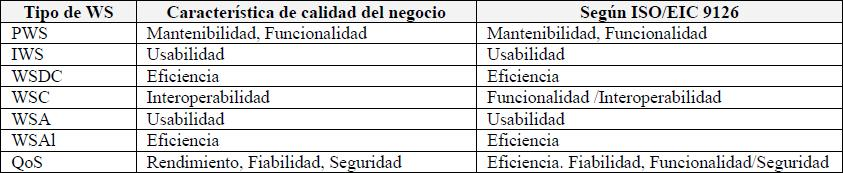
\includegraphics[width=0.9\textwidth]{CalidadSW}
%  \caption{Características de calidad asociadas al tipo de Servicio Web}
%  \label{fig4:SW}
%\end{figure}



%\begin{quotation}
Para poder implementar un servicio Web se cuenta con las siguientes tecnologías:
%\end{quotation}

\begin{itemize}\itemsep=0pt
\item  \textbf{Protocolo Simple de Acceso al Objeto (SOAP).-} Es un estándar de la World Wide Web Consortium (W3C) que describe un formato de mensaje (basado en XML) y mecanismos para intercambiar información entre aplicaciones, en un ambiente distribuido y descentralizado.
\item  \textbf{Lenguaje de Definición del servicio Web (WSDL).-} Es un estándar de la W3C que define un lenguaje basado en XML que permite describir la interfaz, formas de acceso y ubicación de un Servicio Web.
\item  \textbf{Universal Descripción, Descubrimiento e Integración (UDDI).-} Estándar de la
Advancing Open Standards for the Information Society (OASIS) que provee una forma estándar de publicar, categorizar y buscar Servicios Web.
\end{itemize}




%%%%%%%%%%%%%%%%%%%%%%% BIBLIOGRAFIA
\newpage
\bibliographystyle{abbrv}
%\bibliographystyle{unsrt}
%\bibliographystyle{apalike}
\bibliography{bibliografia}


\end{document}

